%%%%%%%%%%%%%%%%%%%%%%%%%%%%%%%%%%%%%%%%%%%%%%%%%%%%%%%%%%%%%%%%%%%%%%%%%%%%%%%%%%%%%
%																					%
%	TRABAJO: Proyecto Integrador													%
%																					%
%		Titulo: 	Desarrollo de IP cores con procesamiento de Redes de Petri 		%
%					Temporales para sistemas multicore en FPGA						%
%																					%
%		Autores:	Juli�n Nonino													%
%					Carlos Renzo Pisetta											%
%		Director:	Orlando Micolini												%
%																					%
%	Parte: Marco Te�rico															%
%	Capitulo: Redes de Petri														%	
%	Archivo: chap_redes_de_petri.tex												%
%																					%
%%%%%%%%%%%%%%%%%%%%%%%%%%%%%%%%%%%%%%%%%%%%%%%%%%%%%%%%%%%%%%%%%%%%%%%%%%%%%%%%%%%%%

% Path Imagenes: ./marco_teorico/redes_de_petri/img
% Nombre predeterminado imagenes: petrixx
%	xx es el numero de imagen

\chapter{Redes de Petri}
	\label{chap:chap_redes_de_petri}

	En este cap�tulo se realizar� una introducci�n a las Redes de Petri, explicando los elementos que la componen,
	sus propiedades, el grafo de alcanzabilidad de marcados, invariantes de plazas y transiciones, trampas y sifones.
	Tambi�n, se muestra la ecuaci�n de estado de una Red de Petri y c�mo es posible ejecutar la red a partir de ella.
	Luego, se presentar�n extensiones que permiten formar las Redes de Petri con Arcos Inhibidores, y las Redes de 
	Petri Temporales. Para estas �ltimas, se detallar�n las dos sem�nticas de tiempo posibles, Redes de Petri con 
	Tiempo y Redes de Petri Temporizadas.

	El objetivo de este cap�tulo es instruir brevemente al lector sobre Redes de Petri, brindando los conocimientos 
	b�sicos para la comprensi�n de otros cap�tulos de este trabajo.
	
	% Introduccion
		%%%%%%%%%%%%%%%%%%%%%%%%%%%%%%%%%%%%%%%%%%%%%%%%%%%%%%%%%%%%%%%%%%%%%%%%%%%%%%%%%%%%%
%																					%
%	TRABAJO: Proyecto Integrador													%
%																					%
%		Titulo: 	Desarrollo de IP cores con procesamiento de Redes de Petri 		%
%					Temporales para sistemas multicore en FPGA						%
%																					%
%		Autores:	Juli�n Nonino													%
%					Carlos Renzo Pisetta											%
%		Director:	Orlando Micolini												%
%																					%
%	Parte: Marco Teorico															%
%	Capitulo: Redes de Petri														%
%	Seccion: Introduccion															%	
%	Archivo: introduccion.tex														%
%																					%
%%%%%%%%%%%%%%%%%%%%%%%%%%%%%%%%%%%%%%%%%%%%%%%%%%%%%%%%%%%%%%%%%%%%%%%%%%%%%%%%%%%%%

% Path Imagenes: ./marco_teorico/redes_de_petri/img
% Nombre predeterminado imagenes: petrixx
%	xx es el numero de imagen

\section{Introducci�n}
	\label{sec:introduccion_petri}

	Una Red de Petri o Petri Net es un modelo gr�fico, formal y abstracto para describir y analizar el flujo de 
	informaci�n. Conforma una herramienta matem�tica que puede aplicarse especialmente a los sistemas paralelos 
	que requieran simulaci�n y modelado de la concurrencia en los recursos compartidos. Las Redes de Petri (PN) 
	est�n asociadas con la teor�a de grafos y se pueden considerar como aut�matas formales y generadores de 
	lenguajes formales \cite{diaz_petri}.
		
	Las Redes de Petri constan de cuatro componentes fundamentales.
	\begin{itemize}
		\item \textbf{Plazas}: Las plazas de una Red de Petri, permiten representar el estado del sistema. 
			Podr�an definirse como variables de estado que toman valores enteros (cantidad de \emph{tokens}).
			Se representan con un c�rculo.
		\item \textbf{Transiciones}: Son representadas con un rect�ngulo. Representan el conjunto de sucesos
			que hacen que el estado del sistema cambie.
		\item \textbf{Arcos}: Los arcos indican las conexiones entre lugares y transiciones. Nunca unen dos 
			lugares o dos transiciones en forma sucesiva. Pueden entrar o salir varios arcos de una misma 
			transici�n o de un mismo lugar.
			Los arcos tienen asociado un \emph{peso} que indica la cantidad de tokens que se consumen o generan al 
			atravesarlo. El disparo de una transici�n retira tantos tokens de cada uno de sus lugares de entrada 
			como lo indican los pesos de los arcos conectores y a�ade los tokens a sus lugares de salida como lo 
			indican los pesos de los arcos de salida.
		\item \textbf{Tokens}: Los tokens representan el valor espec�fico de la condici�n o estado. Son graficados 
			como un punto negro, un n�mero natural o cero dentro de una plaza.
	\end{itemize}

	La \ref{fig:Petri01} muestra c�mo son representados en el grafo de una Red de Petri los conceptos antes mencionados.
	\begin{figure}[H]
		\centering
		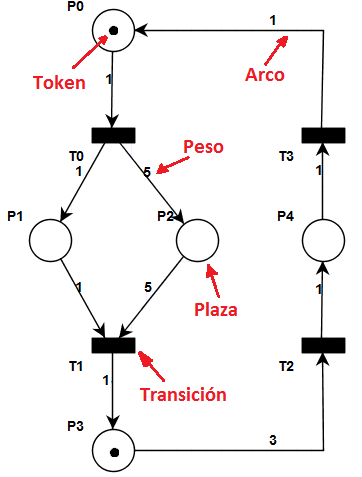
\includegraphics[width=.35\linewidth]{./marco_teorico/redes_de_petri/img/Petri01}
		\caption{Ejemplo de Red de Petri}
		\label{fig:Petri01}
	\end{figure}

	\subsection{Estructura de una Red de Petri}
		Una Red de Petri Marcada queda definida como una 5-tupla de la siguiente manera:
		\begin{center}
			$PN = \{P, T, I^-, I^+, m_0\}$ 
		\end{center}
		Donde:
		\begin{itemize}
			\item $\boldsymbol{P = \{p_1, p_2, p_3 \ldots p_m\}}$, conjunto de $m$ lugares con $m$ finito y 
				distinto de cero.
				Para el ejemplo de la \ref{fig:Petri01} la cantidad de plazas es cinco y se
				tiene que: ${P = \{p_1, p_2, p_3, p_4, p_5\}}$
			\item $\boldsymbol{T = \{t_1, t_2, t_3 \ldots t_n\}}$, conjunto de $n$ transiciones con $n$ finito y 
				distinto de cero. En el ejemplo de la Figura \ref{fig:Petri01} hay cuatro transiciones y se 
				tiene que: ${T = t_1, t_2, t_3\}}$
			\item \textbf{$\boldsymbol{I}$, matriz de incidencia}. Esta matriz es de dimensiones $m�n$, representa los pesos
			 	de los arcos, siendo sus valores positivos cuando el arco va desde una transici�n hacia una plaza 
			 	y negativos los inversos.
				As� mismo esta matriz de incidencia debe separarse en dos para representar la estructura. Estas dos 
				matrices son:
				\begin{description}
					\item [$\boldsymbol {I-}$] Matriz de incidencia negativa. Esta matriz es de dimensiones $m�n$, 
						representa los pesos de los arcos que ingresan desde los lugares de P a las transiciones 
						de T.
					\item [$\boldsymbol {I+}$] Matriz de incidencia positiva. Esta matriz es de dimensiones $m�n$, 
						representa los pesos de los arcos que salen desde las transiciones de T hacia los lugares 
						de P. 
					\end{description}
				Para una red con $m$ plazas y $n$ transiciones, la matriz de incidencia es de tama�o $m�n$, sus 
				elementos $a_{ij}$ son:
				\begin{equation}
					\begin{matrix}
						\forall p_i \in P \wedge \forall t_j\in T \Rightarrow a_{ij}=\;
						\begin{cases} 
							\begin{matrix} 	0 		& si \; entre \; p_i \; y \; t_j\\ 
					 						  		&	 \;	no \; existen\; arcos\\
											W_{ij} 	& si \; p_i \; es \; plaza\\
												 	& de \; salida \; de \; t_j\\
											-W_{ij} & si \; p_i\; es \; plaza\\
											 		& de \; entrada \; de \; t_j 
							\end{matrix}
						\end{cases}
					\end {matrix}
					\label{eq:definicionincidencia}
				\end{equation}
				
				Para la red de la Figura \ref{fig:Petri01} la matriz de incidencia tiene la siguiente forma
				
				\begin{center}
					\begin{tabular}{c c}
						%Primer fila - Columna 1
							$I^+ = \begin{bmatrix}
 						  				0 & 0 & 0 & 1 \\
 						  				1 & 0 & 0 & 0 \\
   						  				5 & 0 & 0 & 0 \\
   						  				0 & 1 & 0 & 0 \\
   						  				0 & 0 & 1 & 0 \\
   									\end{bmatrix}$
   						&
   						%Primer fila - Columna 2
							$I^- = \begin{bmatrix}
 						  				1 & 0 & 0 & 0 \\
 						  				0 & 1 & 0 & 0 \\
   						  				0 & 5 & 0 & 0 \\
   						  				0 & 0 & 3 & 0 \\
   						  				0 & 0 & 0 & 1 \\
   									\end{bmatrix}$
   				 		\\
   				 		Matriz de incidencia positiva & Matriz de incidencia negativa
   				 		\\
   				 		\\
						% Segunda fila
						\multicolumn{2}{c}
						{	$I = \begin{bmatrix}
 						  			-1 & 0 & 0 & 1 \\
 						  			1 & -1 & 0 & 0 \\
   						  			5 & -5 & 0 & 0 \\
   						  			0 & 1 & -3 & 0 \\
   						  			0 & 0 & 1 & -1 \\
   								\end{bmatrix}$  
   						}
						\\
						\multicolumn{2}{c}{Matriz de incidencia}
					\end{tabular}
				
				\end{center}
						
			\item $\boldsymbol {m_0}$ es el \textbf{marcado inicial} de la red, un vector de asignaci�n de 
				tokens a las plazas de la red, de esta forma se define la configuraci�n inicial de los tokens 
				de la red. Por ejemplo puede definirse el marcado de una plaza como $m(i)$, esto indica la 
				cantidad de tokens ubicados en la plaza $i$.
		 		Para el ejemplo anterior, resulta: $m_0 = \begin{bmatrix}
 						  									1 & 0 & 0 & 1 & 0
 						  									\end{bmatrix}^T$
		\end{itemize}
	
	\subsection{Ejecuci�n de una Red de Petri}
	
		El comportamiento din�mico de una red de Petri est� definido por la sensibilizaci�n y el disparo 
		de sus transiciones.
	
		\subsubsection{Transici�n sensibilizada}
			Se dice que una transici�n $t_j$ est� sensibilizada si y s�lo si todas las plazas de entrada a la 
			transici�n tienen una cantidad de tokens igual o mayor al peso indicado por el arco que la une con 
			la transici�n.
			Formalmente:
			\begin{equation}
				\forall p_i\in I^-(t_j)/ m(p_i)\geq W_{ij}
				\label{eq:transiciion_sensibilizada}
			\end{equation}
			
			Siendo $W_{ij}$ el peso del arco que une la plaza $i$ con la transici�n $j$.				
		
		\subsubsection{Disparo de una transici�n}
		
			El disparo de una transici�n es lo que provoca que el estado (marcado) de una Red de Petri cambie. 
			La funci�n disparo (d) de una transici�n $t_j$  se define de la siguiente manera.
			\begin{equation}
				\begin{matrix}
					d(m_k,t_j )\Rightarrow m_{k+1} (p_i)= \;
					\begin{cases} 
						\begin{matrix} 	m_k (p_i )-W_{ij} & \forall p_i \in I^-(t_j)\\
										m_k (p_i )+W_{ij} & \forall p_i \in I^+(t_j)\\
										m_k (p_i ) & para\; el\; resto\; de\; los\; casos 
						\end{matrix}
					\end{cases}
				\end {matrix}
				\label{eq:disparo}
			\end{equation}
			Donde:
			\begin{itemize}
			  	\item $m_k$ es el marcado actual de la red 
  			  	\item $m_{k+1}$ es el marcado que tomara la red luego del disparo.
  			  	\item $W_{ij}$ son los elementos de la matriz de incidencia \emph{I}.
			\end{itemize}
					
		\subsubsection{Ecuaci�n de estado de una Red de Petri}
			\label{subsubsec:ecuacion_estado_petri}
			
			La ecuaci�n de estado determina el estado de la Red de Petri a cada instante, queda definida a 
			partir de la matriz de incidencia y un vector de disparo que indica la transici�n o transiciones 
			que deben ser disparadas.
			\begin{equation}
				m_{k+1} = m_k + I � d_k
				\label{eq:ecuacion_estado_uno}
			\end{equation}
			
			Siendo $d$, un vector cuya dimensi�n es la cantidad de transiciones y su funci�n, indicar cu�l o 
			cu�les transiciones se desean disparar.
			
			Si se parte desde el marcado inicial $m_0$, se puede aplicar sucesivamente la ecuaci�n de estado para 
			llegar al estado $i$. De �sta manera, se deduce la siguiente ecuaci�n:
			\begin{equation}
				m_i = m_0 + I � \sum_{k=1}^{i} d_k
				\label{eq:ecuacion_estado_dos}
			\end{equation}
				
	
	
	% Propiedades de las Redes de Petri
		%%%%%%%%%%%%%%%%%%%%%%%%%%%%%%%%%%%%%%%%%%%%%%%%%%%%%%%%%%%%%%%%%%%%%%%%%%%%%%%%
%	TRABAJO: Proyecto Integrador
%		Titulo: 	Desarrollo de IP cores con procesamiento de Redes de Petri 	
%					Temporales para sistemas multicore en FPGA					
%		Autores:	Juli�n Nonino												%					Carlos Renzo Pisetta										%		Director:	Orlando Micolini											
%%%%%%%%%%%%%%%%%%%%%%%%%%%%%%%%%%%%%%%%%%%%%%%%%%%%%%%%%%%%%%%%%%%%%%%%%%%%%%%%

% Path im�genes: ./marco_teorico/redes_de_petri/img
% Nombre predeterminado im�genes: petrixx
%	xx es el numero de imagen

\section{Propiedades de las Redes de Petri}
	\label{sec:propiedades_petri}

	Las Redes de Petri tienen propiedades especiales que se detallar�n a continuaci�n.
	
	\subsection{Redes de Petri limitadas}
		
		Sea la Red de Petri $PN = {P, T, I^-, I^+, m_0}$, se dice que una plaza $p$ es \textbf{\emph{k-limitada}} si existe un valor $k$ tal que para todo marcado $m$ perteneciente al conjunto de marcados de la Red de Petri $PN$ se cumple que el valor de marcado de la plaza $p$ es menor o igual que $k$.
		\begin{equation}
			\exists k / \forall m \in marcados(PN) : m(p) \leq k
			\label{eq:red_limitada}
		\end{equation}
		
		El arreglo $marcados(PN)$ representa todos los marcados posibles de la Red de Petri. Se dice que una Red de Petri es \emph{k-limitada} si todas sus plazas son \emph{k-limitadas}.
		
	\subsection{Redes de Petri seguras}
	
		Se dice que una red de Petri PN es \textbf{\emph{segura}} si y s�lo si todas sus plazas son \textbf{\emph{1-limitadas}}. Esto implica que una transici�n no puede ser disparada si alguna de sus plazas de llegada est� ocupada.
		
	\subsection{Redes de Petri c�clicas}
			
		Se dice que una Red de Petri es \textbf{\emph{c�clica}} si existe siempre una sucesi�n de marcados que lleve desde cualquier marcado $m$ al marcado inicial $m_0$.
	
	\subsection{Redes de Petri repetitivas}

		Se dice que una Red de Petri es \textbf{\emph{repetitiva}} si existe siempre una secuencia de disparos que lleve desde un marcado $m$ hasta el mismo marcado $m$.

	\subsection{Redes de Petri conservativas}

		Una Red de Petri es \textbf{\emph{conservativa}} si se cumple que para todo marcado $m$ perteneciente al conjunto de marcados de la red, la cantidad de marcas de $m$ es igual a la cantidad de marcas de $m_0$. Es decir, se conserva la cantidad de tokens.

	\subsection{Propiedad de vivacidad (liveness)}

		Se dice que una Red de Petri esta \textbf{\emph{viva}} si y s�lo si en todo momento sus transiciones pueden ser disparadas o si existe una secuencia de disparos v�lidos que lleven a que la transici�n pueda dispararse. 

	\subsection{Propiedades de bloqueo (deadlock)}
	
		Un \textbf{\emph{bloqueo}} en una Red de Petri implica que una transici�n nunca podr� ser disparada independientemente de la secuencia de disparos que se aplique. Recordando la propiedad anterior, se puede decir que una Red de Petri viva garantiza la ausencia de bloqueos. Este concepto est� sustentado en la ausencia de \emph{marcados sumideros}. Un marcado sumidero es aquel marcado a partir del cual ninguna transici�n puede ser disparada.
		
	\subsection{Alcanzabilidad}

		La alcanzabilidad determina si un marcado $m$ es alcanzable desde un marcado inicial $m_0$, es decir, determina si $m$ pertenece al conjunto de marcados de la Red de Petri. Se dice que un marcado $m$ es alcanzable desde $m_0$ si y s�lo si existe una secuencia de disparos que lleven desde $m_0$ hasta $m$. Para determinar si un marcado $m$ es alcanzable, se utiliza la ecuaci�n de estado de una Red de Petri de la siguiente manera:
		\begin{equation}
			m = m_0 + I � \sigma
			\label{eq:alcanzabilidad}
		\end{equation}
		D�nde $\sigma$ es una secuencia de disparos.
				
		Si no fuera posible encontrar una secuencia de disparos, se dice que el marcado $m$ es \emph{inalcanzable}. Si existieran m�ltiples soluciones, es decir, varias secuencias de disparos posibles para alcanzar el marcado $m$, se dice que la Red de Petri se comporta de manera \emph{NO determin�stica}. Hay que notar que la soluci�n de la ecuaci�n no indica el orden en que las transiciones deben ser disparadas, por lo que, �ste debe ser encontrado ejecutando todas las secuencias posibles. Por ello, es posible que a pesar de encontrar una secuencia de disparos, no exista un ordenamiento de los mismos que permita alcanzar la marca $m$ y sea aplicable a la Red de Petri en cuesti�n.
		
		\subsubsection{Grafo de alcanzabilidad}
				
			El grafo de alcanzabilidad de una Red de Petri representa el conjunto de todos los marcados alcanzables desde el marcado inicial $m_0$. Consiste en un grafo en forma de �rbol en el que cada nodo es un marcado alcanzable de la red y se conectan mediante arcos etiquetados con la transici�n que se dispara para pasar de un marcado a otro.
			
			Partiendo del estado inicial $m_0$ se generan todos los estados alcanzables desde �ste mediante un disparo de cada una de las transiciones sensibilizada. A partir de cada estado, se vuelve a repetir el proceso, apareciendo, en consecuencia, un grafo en forma de �rbol que representa todos los estados del sistema.
			
			Por ejemplo, sea la siguiente Red de Petri, se plantear� el grafo de alcanzabilidad de la misma.
				
			\begin{figure}[H]
				\centering
				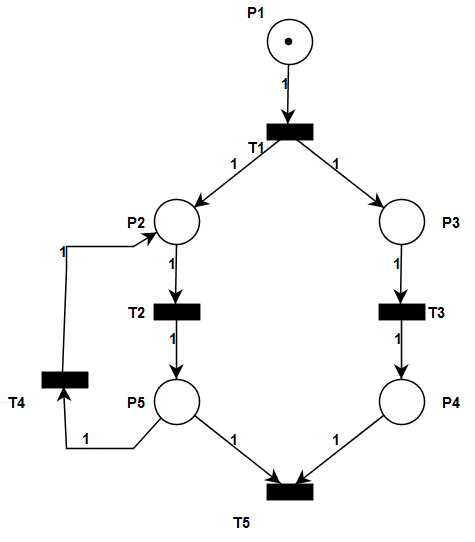
\includegraphics[width=0.5\linewidth]{./marco_teorico/redes_de_petri/img/Petri02}
				\caption{Red de Petri de Ejemplo para Grafo de alcanzabilidad}
				\label{fig:Petri02}
			\end{figure}
				
			El grafo de alcanzabilidad de la red de la Figura \ref{fig:Petri02}, comenzar�a de la siguiente manera:
			\begin{figure}[H]
				\centering
				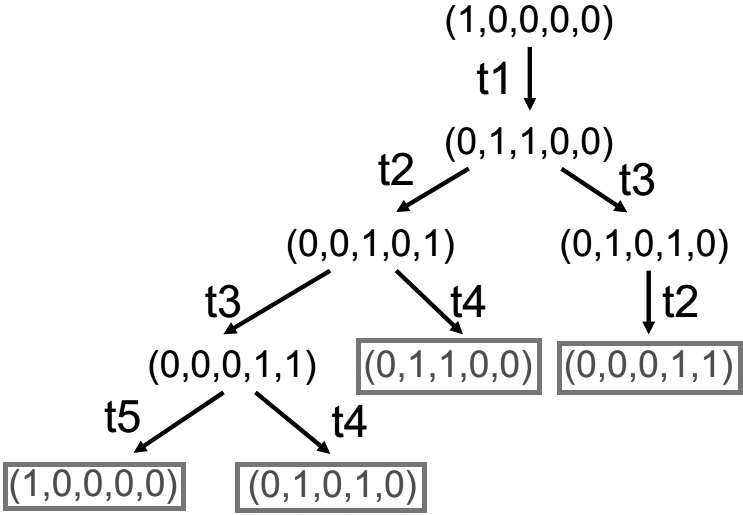
\includegraphics[width=0.65\linewidth]{./marco_teorico/redes_de_petri/img/Petri03}
				\caption{Ejemplo de grafo de alcanzabilidad}
				\label{fig:Petri03}
			\end{figure}
			El proceso se detiene en los marcados repetidos, que en la Figura \ref{fig:Petri03} aparecen recuadrados.

	
	% An�lisis estructural de Redes de Petri
		%%%%%%%%%%%%%%%%%%%%%%%%%%%%%%%%%%%%%%%%%%%%%%%%%%%%%%%%%%%%%%%%%%%%%%%%%%%%%%%%
%	TRABAJO: Proyecto Integrador
%		Titulo: 	Desarrollo de IP cores con procesamiento de Redes de Petri 	
%					Temporales para sistemas multicore en FPGA					
%		Autores:	Juli�n Nonino												%					Carlos Renzo Pisetta										%		Director:	Orlando Micolini											
%%%%%%%%%%%%%%%%%%%%%%%%%%%%%%%%%%%%%%%%%%%%%%%%%%%%%%%%%%%%%%%%%%%%%%%%%%%%%%%%

% Path im�genes: ./marco_teorico/redes_de_petri/img
% Nombre predeterminado im�genes: petrixx
%	xx es el numero de imagen

\section{An�lisis estructural de Redes de Petri}
	\label{sec:analisis_estructural}

	Las propiedades de una Red de Petri pueden ser demostradas construyendo el grafo de alcanzabilidad de la misma. Sin embargo, el tama�o de este grafo crece exponencialmente con el n�mero de plazas.
	
	El an�lisis estructural de una Red de Petri, hace posible demostrar algunas de las propiedades de la red sin necesidad de realizar el grafo de alcanzabilidad.
	
	Existen dos t�cnicas principales, los \textbf{invariantes} y las \textbf{trampas (traps)}.
	
	\subsection{Invariantes de plazas y transiciones}
		\label{subsec:invariantes}
	
		\subsubsection{Definiciones}
			
			El efecto de una secuencia de disparos en la ecuaci�n  de estado de una Red de Petri est� determinado por la matriz de incidencia $I$ y el vector de ocurrencias de transiciones en la secuencia de disparo.
			
			Sea $\sigma\in T^*$ una secuencia de disparos que lleva a una Red de Petri desde el estado $m$ hasta el estado $m_{i+1}$ entonces se puede decir que:
			\begin{itemize}
  				\item La secuencia $\sigma$ tiene asociado un vector $\vec{\sigma}\in \mathbb{N}^T$ (siendo $T$ la cantidad de transiciones de la red) llamado vector de ocurrencia tal que $\vec{\sigma}$ representa la cantidad de ocurrencias de $t$ en la secuencia $\sigma$.
	  			\item La ecuaci�n de estado resulta:
	  					\begin{equation*}
	  						m_(i+1) = m_i + I � \vec{\sigma}
	  					\end{equation*}
				\end{itemize}
			
		\subsubsection{Invariantes}		
			
			Con la ayuda de la ecuaci�n anterior, se buscan cantidades invariantes que permitan analizar estructuralmente a la Red de Petri. En particular, se trabajar� con los canceladores de la matriz de incidencia $I$.
			
			Sea $P$ la cantidad de plazas de una Red de Petri y $T$ la cantidad de transiciones, las cancelaciones de la matriz $I$ generan cuatro vectores:
			\begin{itemize}
				\item \underline{P-flow}
			  		\\
				  	Es un vector no nulo $ x\in \mathbb{Z}^P$ que satisface la siguiente ecuaci�n:
				  	\begin{equation}
						x^t � I = \vec{0} 
						\label{eq:pflow}
					\end{equation} 
					
				\item \underline{P-semiflow}
					\\
				  	Es un vector no nulo $ x\in \mathbb{N}^P$ que satisface la siguiente ecuaci�n:
				  	\begin{equation}
						x^t � I = \vec{0} 
						\label{eq:psemiflow}
					\end{equation}
				\item \underline{T-flow}
					\\
				  	Es un vector no nulo $ u\in \mathbb{Z}^P$ que satisface la siguiente ecuaci�n:
				  	\begin{equation}
						u^t � I = \vec{0} 
						\label{eq:tflow}
					\end{equation} 
				\item \underline{T-semiflow}
					\\
				  	Es un vector no nulo $ u\in \mathbb{N}^P$ que satisface la siguiente ecuaci�n:\\
				  	\begin{equation}
						u^t � I = \vec{0} 
						\label{eq:tsemiflow}
					\end{equation}
			\end{itemize}
  
			Un vector \textbf{P-flow} es una suma ponderada de las plazas con coeficientes enteros. Provee una transformaci�n desde el marcado de un conjunto de plazas a un n�mero entero.
						
			Un \textbf{P-semiflow} es una suma ponderada de las plazas con coeficientes naturales.
						
			Los vectores P-flow y P-semiflow son llamados \textbf{invariantes de plazas} o \textbf{P-invariantes}.
			\\
			
			Los \textbf{T-semiflows} pueden ser obtenidos como el vector de ocurrencia de una secuencia de disparos, mientras que los \textbf{T-flows} pueden ser obtenidos a partir de la diferencia entre dos vectores de ocurrencia.
			
			Los vectores T-flow y T-semiflow son llamados \textbf{invariantes de transiciones} o \textbf{T-invariantes}.
			\\
			
			\begin{raggedright}
				\textbf{\emph{Proposiciones}}
			\end{raggedright}
			
			\begin{enumerate}
  				\item Sea $x$ un vector \emph{P-flow} y $\sigma$ una secuencia de disparos que lleva desde el estado $m_i$ hasta el estado $m_{i+1}$ entonces:
  					\begin{equation}
						x^t � m_i = x^t � m_{i+1} 
						\label{eq:efectopflow}
					\end{equation}
					
					Esto se demuestra con la ecuaci�n de estado:
  						\begin{equation*}
  							\begin{array}{c}
  								 m_{i+1} = m_i + I � \vec{\sigma}
  								 \\
  								 x^t � m_{i+1} = x^t � (m_i + I � \vec{\sigma})
  								 \\
  								 x^t � m_{i+1} = x^t � m_i + x^t � I �\vec{\sigma}
  							\end{array}
  						\end{equation*}	
  					
  					Luego, como $x^t � I = \vec{0}$ entonces:
  						\begin{equation*}
  							x^t � m_{i+1} = x^t � m_i
  						\end{equation*}
  				
  				\item Sea $u$ un vector \emph{T-semiflow} y $\sigma$ una secuencia de disparos tal que 
  					$\sigma = u$, entonces:
  					\begin{equation}
						m_i\xrightarrow{\;\sigma\;} m_{i+1}\Rightarrow m_i = m_{i+1}
						\label{eq:efectopsemiflow}
					\end{equation}
					
					En otras palabras, $\sigma$ es una secuencia repetitiva y estacionaria.
					
					La afirmaci�n anterior se demuestra con la ecuaci�n de estado de la siguiente manera:
	  					\begin{equation*}
	  						m_{i+1} = m_i+I � \vec{\sigma}
	  					\end{equation*}
  					
  					Dado que $\vec{\sigma} = u$\\
	  					\begin{equation*}
	  						m_{i+1} = m_i + I � u
	  					\end{equation*}
  					
  					Luego, como $I � u = \vec{0}$ entonces:
  					\begin{equation*}
  						m_{i+1} = m_i
  					\end{equation*}
  						
  				\item Sea $u$ un vector \emph{T-flow} y $\sigma_1$ y $\sigma_2$ dos secuencias de disparos tal que $\sigma_1 - \sigma_2 = u$, entonces:
  					\begin{equation}
						m\xrightarrow{\;\;\sigma_1\;\;} m' 
						\wedge 
						m\xrightarrow{\;\;\sigma_2\;\;} m''
						\Rightarrow
						m' = m''
						\label{eq:efectotsemiflow}
					\end{equation}
					
					Con la ecuaci�n de estado, se demuestra la proposici�n anterior de la siguiente forma:
					\begin{equation*}
						m' = m + I � \vec{\sigma_1}
						m'' = m + I � \vec{\sigma_2}
					\end{equation*}
					
					Haciendo:
					\begin{equation*}
						\begin{array}{c}
							m' - m'' = (m + I � \vec{\sigma_1}) - (m + I � \vec{\sigma_2}) \\
							m' - m'' = m + I � \vec{\sigma_1} - m - I � \vec{\sigma_2} \\
							m' - m'' = I � \vec{\sigma_1} - I � \vec{\sigma_2} \\
							m' - m'' = I � (\vec{\sigma_1} - \vec{\sigma_2}) 
						\end{array}
					\end{equation*}
					
					Dado que $\vec{\sigma_1} - \vec{\sigma_2} = u$
					\begin{equation*}
						m' - m'' = I � u	
					\end{equation*}							 
  					
  					Luego, como $ I � u = \vec{0}$ entonces
  					\begin{equation*}
  						m' - m'' = \vec{0}
  					\end{equation*}	
			\end{enumerate}
			
		\subsubsection{Invariantes de Transiciones}
			
			Los vectores \emph{T-flow} y los \emph{T-semiflow} son \textbf{invariantes de transiciones} o \textbf{T-invariantes}. En particular, los vectores \emph{T-semiflow} indican posibles bucles (loops) en la red. Es decir, una secuencia de disparos que tenga asociado un invariante de transici�n, vuelve al mismo marcado desde el que parti�. Por ejemplo, sea la siguiente Red de Petri, el vector:
			\begin{figure}[H]
				\begin{minipage}{0.5\textwidth}
					\centering 
					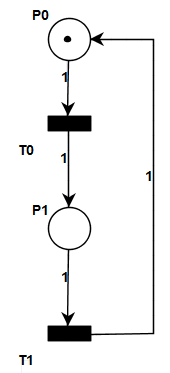
\includegraphics[width=0.3\textwidth]{./marco_teorico/redes_de_petri/img/Petri04}
					\caption{Ejemplo para T-invariantes} 
					\label{fig:ej_tinv}
				\end{minipage}
				\hfill
				\begin{minipage}{0.5\textwidth}
					\begin{center}
						$u=\begin{bmatrix}
		 					1 \\
		 					1
		 				\end{bmatrix}$\\
		 			\end{center}
		 			es un invariante de transiciones. Esto se demuestra con la ecuaci�n de estado de la red.
						\begin{center}
							$m=m_0+I�u$\\[3mm]
							$m=\begin{bmatrix}
					 				1 \\
					 				0
					 	   		\end{bmatrix}
					 	   	+ \begin{bmatrix}
					 				-1 &  1 \\
					 				1 & -1
					 			\end{bmatrix}
							� \begin{bmatrix}
					 				1\\
					 				1
					 			\end{bmatrix}$
					 		\\[3mm]
					 		$m=\begin{bmatrix}
					 				1 \\
					 				0
					 			\end{bmatrix}
					 		+  \begin{bmatrix}
					 				0 \\
					 				0
					 		   \end{bmatrix} 
					 		=  \begin{bmatrix}
					 				1 \\
					 				0
					 			\end{bmatrix}$\\	
						\end{center}					 
				\end{minipage}
			\end{figure}
									
		\subsubsection{Invariantes de plazas (p-invariantes)}
			
			Sea una Red de Petri $PN(I, m_0)$ definida por una estructura de red $I$ y un marcado inicial $m_0$, si $x$ es un vector \emph{P-flow} o un \emph{P-semiflow}, se cumple que:
			\begin{equation}
				\forall m \in marcados de PN: x^t � m = x^t � m_0
			\end{equation}
			
			Para todo marcado $m$ perteneciente al conjunto de marcados de la red $PN$ se cumple que el producto de la transpuesta del vector $x$ por cualquier marcado, se mantiene igual al producto con el marcado inicial $m_0$. 
			
			Si el vector $x$ es \emph{P-semiflow}, se dice que $x$ es un \textbf{\emph{invariante positivo}}.
			
			Los invariantes positivos tienen muchas aplicaciones. Por ejemplo, todas las plazas que est�n incluidas en un vector P-invariante se encuentran limitadas al valor de marcado que sumaban al inicio.
			
			Tambi�n, los invariantes de plazas pueden ser utilizados para identificar los estados de los procesos modelados con la Red de Petri y adem�s, para verificar situaciones de exclusi�n mutua. En las Redes de Petri que se presentan a continuaci�n, se ejemplificar�n las aplicaciones antes mencionadas.
			
			Se plantea la Red de Petri de un sistema productor consumidor con un buffer de capacidad limitada.
			\begin{figure}[H]
				\centering
				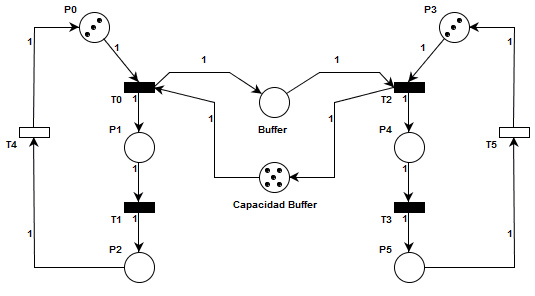
\includegraphics[width=.7\linewidth]{./marco_teorico/redes_de_petri/img/Petri05}
				\caption{Red de Petri para problema Productor-Consumidor}
				\label{fig:Petri05}
			\end{figure}
			
			Los invariantes de plazas pueden ser escritos como ecuaciones que muestran propiedades de la Red de Petri. 
			
			En este ejemplo, los vectores \emph{P-invariantes} son\footnote{Los vectores han sido calculados utilizando la Ecuaci�n \ref{eq:pflow} y la Ecuaci�n \ref{eq:psemiflow}}:
			
			\begin{center}
				\begin{tabular}{c c c c c c c c c}
						& P0	& P1 	& P2 	& P3 	& P4 	& P5 	& Capacidad Buffer 	& Buffer
					\\
					\hline
					1)  & 0 	& 0 	& 0 	& 0 	& 0 	& 0 	& 1 				& 1
					\\
					\hline
					2) 	& 1 	& 1 	& 1 	& 0 	& 0 	& 0 	& 0 				& 0
					\\
					\hline
					3) 	& 0 	& 0 	& 0 	& 1 	& 1 	& 1 	& 0 				& 0\\
					\hline
				\end{tabular}
			\end{center}
			
			Traducidos a ecuaciones resultan:
			\begin{enumerate}
  				\item $M(Capacidad Buffer) + M(Buffer) = 5$
  					\\
					En esta ecuaci�n que se deriva del primer vector \emph{P-invariante}, se puede ver como la cantidad de marcas que se encuentran ubicadas entre las plazas \emph{Capacidad Buffer} y \emph{Buffer}, se mantiene constante. Esto indica, que est�n limitadas.
				\item $M(P0) + M(P1) + M(P2) = 3$
					\\
					Desde el segundo vector \emph{P-invariante}, se obtiene la ecuaci�n anterior. Por esta ecuaci�n, deducimos que las plazas $P0$, $P1$ y $P2$ representan los estados de un proceso. Dado que la cantidad de tokens entre ellas se mantiene constante, esto permite deducir que los tokens van cambiando de estado. Este proceso, se corresponde con el proceso \emph{Productor}.
				\item $M(P3) + M(P4) + M(P5) = 3 $
					\\
					�dem al caso anterior, el hecho de que el numero de tokens se mantenga en las plazas $P3$, $P4$ y $P5$ permite identificar los estados del otro proceso modelado, el proceso \emph{Consumidor}.
			\end{enumerate}
				
			Si el buffer del ejemplo anterior, tuviera que ser accedido con exclusi�n mutua, el modelado del sistema con una Red de Petri resultar�a de la siguiente manera.
			\begin{figure}[H]
				\centering
				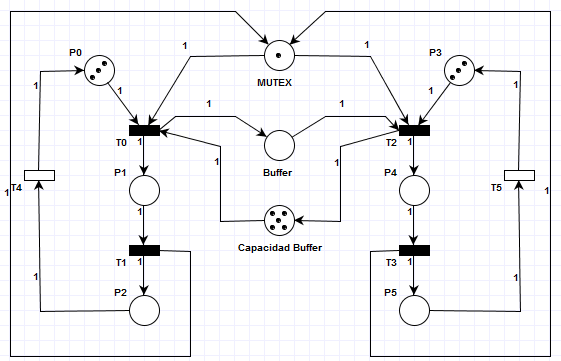
\includegraphics[width=.7\linewidth]{./marco_teorico/redes_de_petri/img/Petri06}
				\caption{Red de Petri para problema Productor-Consumidor con Exclusi�n Mutua}
				\label{fig:Petri06}
			\end{figure}
				
			Obteniendo los vectores \emph{P-invariantes} del sistema se tiene:
			\begin{center}
				\begin{tabular}{c c c c c c c c c c}
						& P0 	& P1 	& P2 	& P3 	& P4 	& P5 	& Capacidad Buffer 	& Buffer 	& MUTEX
					\\
					\hline  
					1) 	& 0 	& 0 	& 0 	& 0 	& 0 	& 0 	& 1 				& 1 		& 0
					\\
					\hline
					2) 	& 1 	& 1 	& 1 	& 0 	& 0 	& 0 	& 0 				& 0 		& 0
					\\
					\hline
					3) 	& 0 	& 0 	& 0 	& 1 	& 1 	& 1 	& 0 				& 0 		& 0
					\\
					\hline
					4) 	& 0 	& 1 	& 0 	& 0 	& 1 	& 0 	& 0 				& 0 		& 1
					\\
					\hline
				\end{tabular}
			\end{center}	
			
			Como se puede notar, se obtuvo un cuarto invariante de plazas adem�s de los que ya aparec�an en el ejemplo anterior. La ecuaci�n de este cuarto invariante es:
			\begin{equation*}
				M(P1) + M(P4) + M(MUTEX) = 1
			\end{equation*}
 
 			Las plazas $P1$ y $P4$ se corresponden con los estados de procesos \emph{Produciendo} y \emph{Consumiendo} respectivamente. El hecho de que aparezcan en un invariante junto con la plaza \emph{MUTEX} indica que la cantidad de tokens entre estas tres plazas no cambia. Dado que el valor constante es \emph{1}, �ste \emph{P-invariante} muestra la exclusi�n mutua entre ambos procesos.
				
	\subsection{Trampas (Traps)}
		\label{subsec:traps}
			
		Para explicar que es un \textbf{\emph{trap}} se presentar� una Red de Petri de ejemplo \cite{muscholl}.
		\begin{figure}[H]
			\centering
			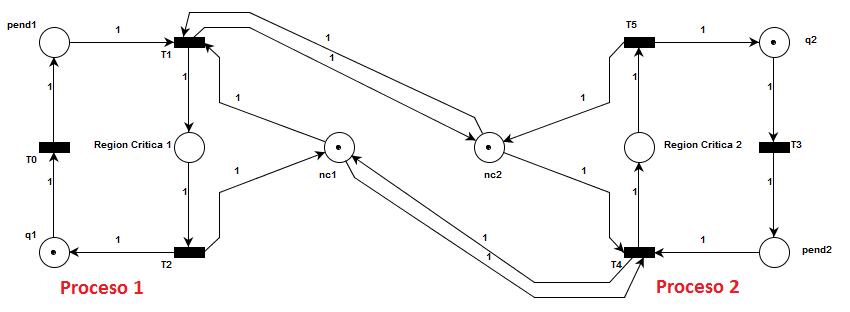
\includegraphics[width=1\linewidth]{./marco_teorico/redes_de_petri/img/Petri07}
			\caption{Ejemplo red de Petri con Traps}
			\label{fig:Petri07}
		\end{figure}		
			
		En la red de la Figura \ref{fig:Petri07}, la idea es conseguir exclusi�n mutua garantizando que un proceso ingrese a su secci�n cr�tica s�lo si el otro proceso no ha ingresado a la suya. Entonces, lo que se desea probar es que para todo marcado $m$ se cumple que:
		\begin{equation*}
			m(RegionCritica1) + m(RegionCritica2) \leq 1
		\end{equation*}
		
		Si se calculan los p-invariantes de la red anterior se tiene:
		\begin{enumerate}
	  		\item $ m(pend1) + m(q1) + m(RegionCritica1) = 1 $
	  		\item $ m(pend2) + m(q2) + m(RegionCritica2) = 1 $
	  		\item $	m(RegionCritica1) + m(nc1) = 1 $
	  		\item $ m(RegionCritica2) + m(nc2) = 1 $
	  	\end{enumerate}
	  		
	  	La red de la Figura \ref{fig:Petri07} tiene arcos bidireccionales entre la plaza $nc1$ y la transici�n $t4$ y entre la plaza $nc2$ y la transici�n $t1$. Los arcos bidireccionales se anulan en la matriz de incidencia produciendo una perdida de informaci�n. Esta perdida de informaci�n hace que los el conjunto de ecuaciones de los p-invariantes no sea suficiente para probar la propiedad de exclusi�n mutua deseada.
		
		Los \textbf{\emph{traps}} en combinaci�n con los \emph{p-invariantes} recuperan la informaci�n perdida debido a los arcos bidireccionales.
		\\

		Sea una Red de Petri $PN = \{P, T, I, m_0\}$ un \textbf{\emph{trap}} es un conjunto de plazas $ S \in P / S^\bullet \subseteq\;^\bullet S$\footnote{$S^\bullet$ representa el conjunto de tokens que se retiran del conjunto de plazas $S$. A su vez, $\;^\bullet S$ representa el conjunto de tokens que se colocan en el conjunto de plazas $S$.}. 
		Esto significa que cada transici�n que remueve tokens de un \emph{trap} debe colocar al menos uno en el \emph{trap}.
			
		Se dice que un \emph{trap} $S$ es marcado en un determinado marcado $m$ si y solo si se cumple que en al menos una plaza $s\in S$ se cumple que $m(s)\geq 1$. Se debe decir que si un \emph{trap} $S$ es marcado en $m_0$, lo ser� tambi�n en todos los marcados alcanzables.
		\\
		
		En el ejemplo de Figura \ref{fig:Petri07}, el conjunto de plazas $S=\{nc1, nc2\}$ es un \emph{trap}.
			
		Las transiciones $t1$ y $t5$ son las que remueven tokens de esas plazas pero tambi�n colocan nuevos tokens en ellas. En el momento inicial, $S$ es un \emph{trap marcado}, entonces, as� lo ser� en todos los marcados alcanzables. De esta manera, se tiene que:
		\begin{equation*}
			m(nc1)+m(nc2)\geq1
		\end{equation*}
		
		Esta nueva inecuaci�n que se a�ade a la descripci�n de la Red de Petri de la Figura \ref{fig:Petri07} permite demostrar la propiedad de exclusi�n mutua. Tomando las ecuaciones de los invariantes 3 y 4:
		\begin{equation*}
			\begin{array}{c}
				m(RegionCritica1) + m(nc1) = 1
				\\
				m(RegionCritica2)+ m(nc2) = 1
			\end{array}
		\end{equation*}		

		Sum�ndolas se obtiene:
		\begin{equation*}
			m(RegionCritica1) + m(nc1) + m(RegionCritica2) + m(nc2) = 2
		\end{equation*}

		Restando la inecuaci�n del trap se obtiene:
		\begin{equation*}
			\begin{array}{c}
				m(RCritica1) + m(nc1) + m(R Critica 2) + m(nc2) - m(nc1) - m(nc2) \leq 1
				\\
				m(RCritica1) + m(R Critica 2) \leq 1
			\end{array}
		\end{equation*}

		Con lo que queda demostrada la propiedad de exclusi�n mutua en las regiones criticas.
			
	\subsection{Sifones(Siphons)}
		\label{subsec:sifon}
		
		Sea una Red de Petri $PN = \{P, T, I, m_0\}$ un \textbf{\emph{sif�n (siphon)}} es un conjunto de plazas $S \in P$ tal que $ ^\bullet S \subseteq S^\bullet$. Esto significa que cada transici�n que coloca tokens en un \emph{siphon} debe remover al menos uno del \emph{siphon}.
			
		Se dice que un \emph{siphon} $S$ es vac�o en un determinado marcado $m$ si y solo si se cumple que para toda plaza $s \in S$ se cumple que $m(s) = 0$. Se debe decir que si un \emph{siphon} $S$ es vac�o en $m_0$, lo ser� tambi�n en todos los marcados alcanzables.

	
	% Clasificaci�n de las Redes de Petri
		%%%%%%%%%%%%%%%%%%%%%%%%%%%%%%%%%%%%%%%%%%%%%%%%%%%%%%%%%%%%%%%%%%%%%%%%%%%%%%%%%%%%%
%																					%
%	TRABAJO: Proyecto Integrador													%
%																					%
%		Titulo: 	Desarrollo de IP cores con procesamiento de Redes de Petri 		%
%					Temporales para sistemas multicore en FPGA						%
%																					%
%		Autores:	Juli�n Nonino													%
%					Carlos Renzo Pisetta											%
%		Director:	Orlando Micolini												%
%																					%
%	Parte: Marco Teorico															%
%	Capitulo: Redes de Petri														%
%	Seccion: Clasificaci�n de las Redes de Petri									%	
%	Archivo: clasificacion.tex														%
%																					%
%%%%%%%%%%%%%%%%%%%%%%%%%%%%%%%%%%%%%%%%%%%%%%%%%%%%%%%%%%%%%%%%%%%%%%%%%%%%%%%%%%%%%

% Path Imagenes: ./marco_teorico/redes_de_petri/img
% Nombre predeterminado imagenes: petrixx
%	xx es el numero de imagen

\section{Clasificaci�n de las Redes de Petri}
	\label{sec:clasificacion}

	Las \textbf{\emph{Redes de Petri (PN)}} se pueden considerar como aut�matas formales y generadores de lenguajes 
	formales. 
	En las siguientes secciones, se analizar�n un conjunto de sintaxis restrictivas que limitan el poder de 
	modelado de las Redes de Petri pero permiten asegurar que el modelo generado cumple con ciertas propiedades.
	\begin{figure}[H]
		\centering
		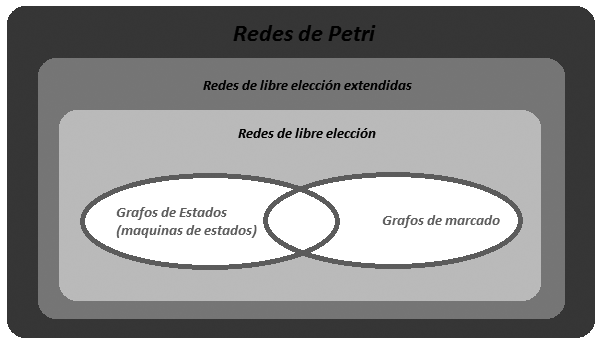
\includegraphics[width=1\linewidth]{./marco_teorico/redes_de_petri/img/Petri08}
		\caption{Subclases de Redes de Petri}
		\label{fig:Petri08}
	\end{figure}
	
	\subsection{Grafos o m�quinas de estado}

		Para representar una m�quina de estados con una Red de Petri, se deben cumplir las siguientes condiciones: 
		cada transici�n tiene un �nico arco de entrada y un �nico arco de salida, las plazas no tienen restricci�n 
		y solo existe un token en toda la red. Esto significa que no puede existir concurrencia, pero si puede 
		haber conflictos. Los conflictos se deben a que como una plaza puede tener muchos arcos de salida, no se 
		puede determinar hacia donde ir� un token. Por ejemplo, en la Figura \ref{fig:Petri09}un token 
		en la plaza $P0$ generar� conflicto entre las transiciones $T0$ y $T1$ dado que no se puede determinar cual 
		debe ser disparada.
		\begin{figure}[H]
			\centering
			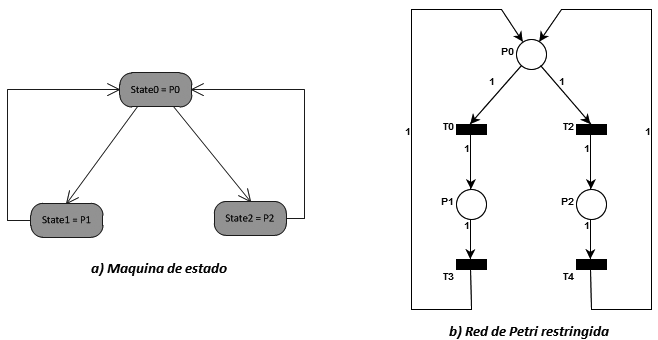
\includegraphics[width=.8\linewidth]{./marco_teorico/redes_de_petri/img/Petri09}
			\caption{Red de Petri restringida a m�quina de estados}
			\label{fig:Petri09}
		\end{figure}
		
		Matem�ticamente, sea $t$ una transici�n perteneciente al conjunto de transiciones $T$ se tiene que:
		\begin{equation}
			\forall t\in T : \mid t\bullet \mid =\mid\bullet t \mid =1
			\label{eq:petri_state_machine}
		\end{equation}
		
		\begin{figure}[H]
			\centering
			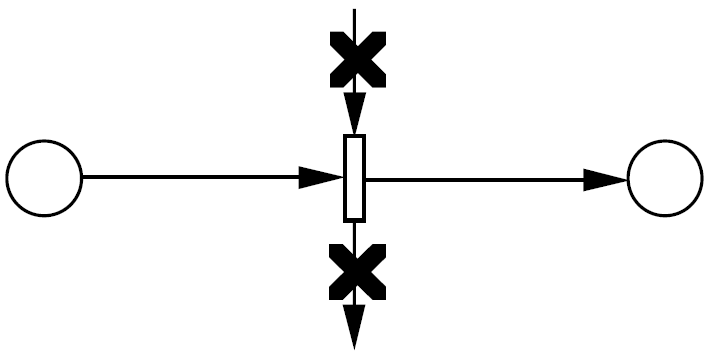
\includegraphics[width=0.25\linewidth]{./marco_teorico/redes_de_petri/img/Petri10}
			\caption{Ilustraci�n de la restricci�n para formar m�quinas de estados}
			\label{fig:Petri10}
		\end{figure}
		
		Generando un modelo con Redes de Petri que cumpla la restricci�n de la Ecuaci�n \ref{eq:petri_state_machine}
		es posible garantizar que el modelo cumple con todas las propiedades propias de las m�quinas de estado, 
		es decir, es conservativa y acotada. La propiedad de vivacidad en este tipo de redes, es simple de 
		demostrar y puede ser calculada de forma lineal con el algoritmo de Tarjan \cite{diaz_petri}.
	
	\subsection{Grafos de marcado}
	
		Para representar un grafo marcado con una Red de Petri debe cumplirse que: una plaza s�lo puede tener un 
		�nico arco de entrada y un �nico arco de salida, las transiciones no tienen restricciones. De esta manera, 
		si es posible que exista concurrencia y adem�s, no existen conflictos dado que un token solo puede 
		disparar una transici�n.
	 
		Matem�ticamente, sea $p$ una plaza perteneciente al conjunto de plazas $P$ se tiene que:
		\begin{equation}
			\forall p\in P : \mid p\bullet \mid =\mid\bullet p \mid =1
			\label{eq:petri_grafo_marcado}
		\end{equation}
		
		\begin{figure}[H]
			\centering
			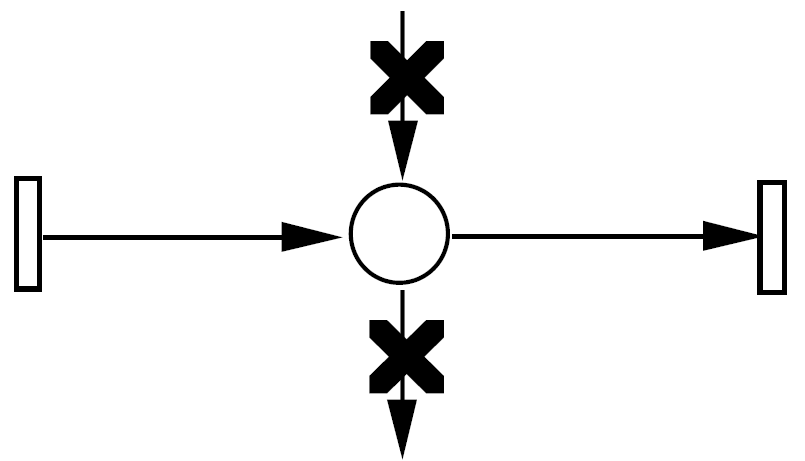
\includegraphics[width=0.25\linewidth]{./marco_teorico/redes_de_petri/img/Petri11}
			\caption{Ilustraci�n de la restricci�n para formar grafos de marcado.}
			\label{fig:Petri11}
		\end{figure}	
		
		Si la Red de Petri es de este tipo, la red es viva (sin deadlock) si y s�lo si cualquier circuito 
		elemental de la red incluye un lugar que inicialmente estaba marcado \cite{diaz_petri}.
		Una red de este tipo, ser� estructuralmente limitada si es fuertemente conectada \cite{diaz_petri}.
	
	\subsection{Redes de libre elecci�n}
		
		En las redes de libre elecci�n, todo arco que va desde una plaza hacia una transici�n, es el �nico arco 
		que sale desde esa plaza o es el �nico que entra en esa transici�n.
		\begin{equation}
			\forall p\in P : (\mid p\bullet \mid\leq 1) \vee (\mid\bullet(p\bullet) \mid =\{1\}
			\label{eq:petri_libre_eleccion}
		\end{equation}
		
		\begin{figure}[H]
			\centering
			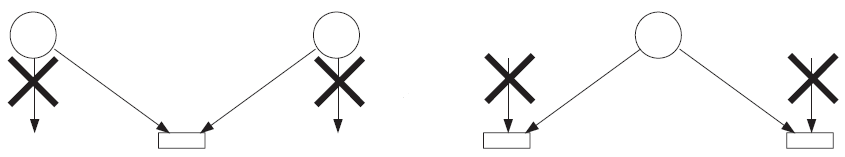
\includegraphics[width=0.7\linewidth]{./marco_teorico/redes_de_petri/img/Petri12}
			\caption{Red de elecci�n libre}
			\label{fig:Petri12}
		\end{figure}	
		
	\subsection{Redes de elecci�n libre extendidas}
	
		Si dos lugares tienen alguna transici�n de salida com�n, entonces ellos tienen todas sus transiciones de 
		salida en com�n, matem�ticamente es equivalente a:
		\begin{equation}
			Sea\;p1\;y\;p2\in P: p1\bullet \cap p2\bullet \neq \phi \Rightarrow \mid p1\bullet \mid=\mid p1\bullet
			\mid
			\label{eq:petri_libre_extendida}
		\end{equation}

		\begin{figure}[H]
			\begin{center}
			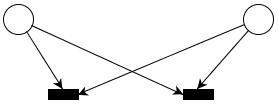
\includegraphics[width=0.3\linewidth]{./marco_teorico/redes_de_petri/img/Petri13}
				\end{center}
				\caption{Red de elecci�n libre extendida}
				\label{fig:Petri13}
		\end{figure}	
		
		De lo definido se puede notar que si una $t$ est� sensibilizada, todas las transiciones estar�n 
		estructuralmente en conflicto. Por lo que se puede elegir libremente entre varias transiciones para disparar.
	  
	
	% Extensiones de las Redes de Petri
		%%%%%%%%%%%%%%%%%%%%%%%%%%%%%%%%%%%%%%%%%%%%%%%%%%%%%%%%%%%%%%%%%%%%%%%%%%%%%%%%
%	TRABAJO: Proyecto Integrador
%		Titulo: 	Desarrollo de IP cores con procesamiento de Redes de Petri 	
%					Temporales para sistemas multicore en FPGA					
%		Autores:	Juli�n Nonino												%					Carlos Renzo Pisetta										%		Director:	Orlando Micolini											
%%%%%%%%%%%%%%%%%%%%%%%%%%%%%%%%%%%%%%%%%%%%%%%%%%%%%%%%%%%%%%%%%%%%%%%%%%%%%%%%

% Path im�genes: ./marco_teorico/redes_de_petri/img
% Nombre predeterminado im�genes: petrixx
%	xx es el numero de imagen

\section{Extensiones de las Redes de Petri}
	\label{sec:extensiones}

	Las Redes de Petri analizadas hasta el momento, pueden ser extendidas agregando arcos inhibidores para considerar la ausencia de tokens como condici�n de sensibilizaci�n de una transici�n (\textbf{\emph{Redes de Petri con Arcos Inhibidores}}), marcas de tiempo para determinar intervalos en los cuales una transici�n puede ser disparada (\textbf{\emph{Redes de Petri con Tiempo}}), o valores de duraci�n en las transiciones(\textbf{\emph{Redes de Petri Temporizadas}}), probabilidades de disparo de transiciones (\textbf{\emph{Redes de Petri Estoc�sticas}}) o cualquier combinaci�n entre ellas.
	
	En la Figura \ref{fig:Petri14}, extra�da del libro \cite{diaz_petri}, se observa la evoluci�n de estas extensiones. Se encuentran marcadas, aquellas que se analizar�n en este trabajo. Las \emph{Redes de Petri con Arcos Inhibidores} est�n incluidas dentro de �tem \emph{Place-transition Petri nets 1962, 1969}.
		
	\begin{figure}[H]
		\centering
		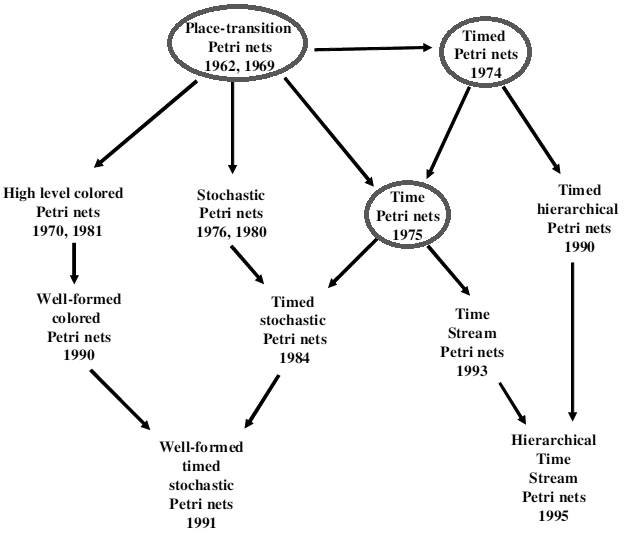
\includegraphics[width=1\linewidth]{./marco_teorico/redes_de_petri/img/Petri14}
		\caption{Extensiones de las Redes de Petri}
		\label{fig:Petri14}
	\end{figure}	
		
	
	% Redes de Petri con Arcos Inhibidores de peso unitario
		%%%%%%%%%%%%%%%%%%%%%%%%%%%%%%%%%%%%%%%%%%%%%%%%%%%%%%%%%%%%%%%%%%%%%%%%%%%%%%%%
%	TRABAJO: Proyecto Integrador
%		Titulo: 	Desarrollo de IP cores con procesamiento de Redes de Petri 	
%					Temporales para sistemas multicore en FPGA					
%		Autores:	Juli�n Nonino												%					Carlos Renzo Pisetta										%		Director:	Orlando Micolini											
%%%%%%%%%%%%%%%%%%%%%%%%%%%%%%%%%%%%%%%%%%%%%%%%%%%%%%%%%%%%%%%%%%%%%%%%%%%%%%%%

% Path im�genes: ./marco_teorico/redes_de_petri/img
% Nombre predeterminado im�genes: petrixx
%	xx es el numero de imagen

\section{Redes de Petri con Arcos Inhibidores de peso unitario}
	\label{sec:arcos_inhibidores}

	En las Redes de Petri vistas anteriormente las transiciones est�n sensibilizadas cuando en las plazas de entrada existe una cantidad igual o mayor de tokens que el peso del arco que los une. Pero, en algunas situaciones, ser�a necesario que una transici�n se encuentre sensibilizada cuando no existan tokens en alguna de sus plazas de entrada. Para este fin existen los arcos inhibidores. Los arcos inhibidores se representan con una l�nea finalizada en un c�rculo. Se debe destacar que s�lo pueden ir desde plazas hacia las transiciones, nunca al rev�s. 

	\subsection{Definici�n matem�tica}

	Una Red de Petri marcada con arcos inhibidores queda definida por una 6-tupla de la siguiente manera:
	\begin{equation*}
		PN={P,T,I^-,I^+,H,m_0}
	\end{equation*}
	
	El elemento nuevo es la matriz \emph{H} llamada \textbf{matriz de inhibici�n} que es una matriz de $p$ filas y $t$ columnas. Siendo $p$ la cantidad de plazas de la red y $t$ la cantidad de transiciones.
	
	Es una matriz binaria, sus elementos solo pueden valer cero (0) o uno (1). Un \emph{uno} en la posici�n $a_{ij}$ indica que la plaza $i$ esta unida a la transici�n $j$ a trav�s de un arco inhibidor. 
	
	\subsection{Transiciones sensibilizadas en Redes de Petri con Arcos Inhibidores}
	
		Se pondr� como ejemplo la siguiente Red de Petri.
		\begin{figure}[H]
			\centering
			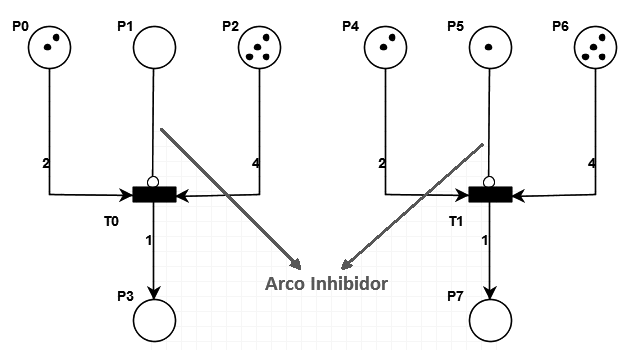
\includegraphics[width=.6\linewidth]{./marco_teorico/redes_de_petri/img/Petri15}
			\caption{ Ejemplo Red de Petri con Arco Inhibidor}
			\label{fig:Petri15}
		\end{figure}	
		
		En la Figura \ref{fig:Petri15}, se ve la representaci�n de un arco inhibidor y c�mo afecta a la transici�n. En la red de la izquierda, la transici�n $T0$ se encuentra sensibilizada mientras que en la red de la derecha la transici�n $T1$ no lo est�, por lo tanto no es posible que se dispare.
	
		Ahora, en una \textbf{\emph{Red de Petri con Arcos Inhibidores}}, se dice que una transici�n esta sensibilizada cuando se cumplen las siguientes condiciones:
		\begin{enumerate}
  			\item $\forall p_i \in I^-(t_j) : m(p_i) \geq W_{ij}$
  				\\
  				Siendo $W_{ij}$ el peso del arco (no inhibidor) que une la plaza $i$ con la transici�n $j$.
			\item Todas las plazas unidas a $t_j$ con arcos inhibidores no deben tener tokens.	
		\end{enumerate}
		
	\subsection{Ejecuci�n de una Red de Petri con Arcos Inhibidores}
			
		La ecuaci�n de estado para una Red de Petri con aros inhibidores toma la siguiente forma:
		\begin{equation}
			m_{i+1} = m_i  + I� \left[ \delta\;and\;f_H (m_i,\delta) \right]
			\label{eq:estado_petri_arcos_inhibidores}
		\end{equation}

		Como se ve, se agrega una funci�n $f$ que depende del marcado actual, del disparo a realizar y, de una funci�n $H$ que determina si una transici�n est� sensibilizada o no de acuerdo a  los arcos inhibidores. Esta funci�n toma solo valores ceros y unos, y al estar en una operaci�n $and$ con el disparo, puede inhibirlo y hacer que no produzca efectos.
		
		A continuaci�n se detalla la funci�n $f$.
		\begin{equation}
			f_H(m_i,\delta) = M_{=0}(m_i)\; nand \;(H � \delta)
			\label{eq:fun_inhibicion}
		\end{equation}
			
		La funci�n $M_{=0}()$ es una funci�n vectorial de $p$ elementos. Donde $p$ es la cantidad de plazas. Cada componente $k$ del resultado de la funci�n $M_{=0}()$ toma su valor de la siguiente ecuaci�n:
		\begin{equation}
			M_{=0}(m)_k =
				\begin{cases} 
					0 & \text{si } m_{ij} \neq 0
					\\
					1 & \text{si } m_{ij}= 0				
				\end{cases}		
			\label{eq:funcion_igual_cero}
		\end{equation}

	
	% Redes de Petri Temporales
		%%%%%%%%%%%%%%%%%%%%%%%%%%%%%%%%%%%%%%%%%%%%%%%%%%%%%%%%%%%%%%%%%%%%%%%%%%%%%%%%
%	TRABAJO: Proyecto Integrador
%		Titulo: 	Desarrollo de IP cores con procesamiento de Redes de Petri 	
%					Temporales para sistemas multicore en FPGA					
%		Autores:	Juli�n Nonino												%					Carlos Renzo Pisetta										%		Director:	Orlando Micolini											
%%%%%%%%%%%%%%%%%%%%%%%%%%%%%%%%%%%%%%%%%%%%%%%%%%%%%%%%%%%%%%%%%%%%%%%%%%%%%%%%

% Path im�genes: ./marco_teorico/redes_de_petri/img
% Nombre predeterminado im�genes: petrixx
%	xx es el numero de imagen

\section{Redes de Petri Temporales}
	\label{sec:redes_temporales}
	
	En los modelos de Redes de Petri descriptos hasta el momento, el tiempo no estaba considerado. 
	
	En el formalismo de Redes de Petri b�sico, o aut�nomo, la abstracci�n del entorno en el que la red evoluciona, incluyendo el tiempo como parte de este entorno, es total. Por lo que existe cierto indeterminismo en cuanto al tiempo: no se especifica cu�ndo se disparar� una transici�n que est� sensibilizada (ni si se disparar� realmente), tampoco cu�l de entre un grupo de transiciones en conflicto ser� la disparada \cite{garcia_izquierdo}.
	
	\newpage
	
	Las distintas interpretaciones con tiempo de las Redes de Petri han tratado de reducir el indeterminismo de distintas maneras. Entre estas interpretaciones est�n:
	\begin{enumerate}
	  	\renewcommand{\theenumi}{\Alph{enumi}}
	  	\item \underline{Redes de Petri Estoc�sticas (Stochastic Petri Net)}
	  		\\
			Se introduce una estimaci�n estoc�stica respecto del instante de disparo de una transici�n.
		\item \underline{Redes de Petri Temporizadas (Timed Petri Net)}
			\\
			Introduce una condici�n de tiempo que establece la duraci�n de la transici�n.
		\item \underline{Redes de Petri con Tiempo (Time Petri Net)}
			\\
			Introducen cotas temporales entre las cuales la transici�n puede o debe ser disparada.
	\end{enumerate}
	
	\begin{figure}[H]
		\centering
		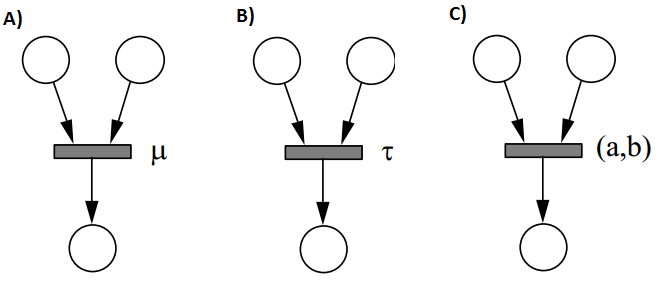
\includegraphics[width=0.9\linewidth]{./marco_teorico/redes_de_petri/img/Petri16}
		\caption{Interpretaciones de Redes de Petri Temporales}
		\label{fig:Petri16}
	\end{figure}
	
	Existen dos maneras de interpretar el par�metro temporal asociado a una transici�n:
	\begin{itemize}
		\item Cuando el par�metro temporal determina el tiempo que ha de transcurrir desde que una transici�n queda sensibilizada hasta que se dispara, procedi�ndose entonces a la retirada y colocaci�n de marcas de forma at�mica, se habla de \textbf{\emph{tiempo de sensibilizaci�n (enabling time)}}. Est� relacionada con las \textbf{\emph{Redes de Petri con Tiempo}} (Red C de la Figura \ref{fig:Petri16}).
		\item El par�metro temporal puede determinar tambi�n el tiempo que debe transcurrir entre la retirada (instant�nea) de marcas de los lugares de entrada, y la colocaci�n (instant�nea) de marcas en los lugares de salida; en �ste caso se habla de tiempo de \textbf{\emph{disparo (firing time)}}. Esto es, el disparo de la transici�n tiene tres fases (retirada de marcas de entrada, disparo, colocaci�n de marcas de salida) y no es at�mico, sino que tienen una duraci�n. Por ello esta interpretaci�n es tambi�n conocida como sem�ntica de duraci�n. Est�n asociadas con las \textbf{\emph{Redes de Petri Temporizadas}} (Red B de la Figura \ref{fig:Petri16}).
	\end{itemize}
	
	Este cap�tulo se centrar� en:
	\begin{itemize}
		\item \textbf{\emph{Redes de Petri con Tiempo:}}
			\\
			En estas redes, cada transici�n tiene asociado un intervalo $[a , b]$ que abarca todas las posibilidades de duraci�n de la actividad que la transici�n modela.
		\item \textbf{\emph{Redes de Petri Temporizadas:}}
			\\
			En estas redes, cada transici�n tiene asociado un par�metro $[a]$ que establece la duraci�n de la transici�n, es decir la duraci�n del intervalo entre que se extraen los tokens de las plazas de entrada y se colocan los tokens en las plazas de salida.
	\end{itemize}
		
	\subsection{Redes de Petri con Tiempo}
		\label{subsec:redes_con_tiempo}
		
		En �sta secci�n se describir�n las \textbf{\emph{Redes de Petri con Tiempo}} como la red \emph{C} de la Figura \ref{fig:Petri16}).
		
		\subsubsection{Definici�n matem�tica}
			Una \emph{Red de Petri Marcada con Tiempo}, se define matem�ticamente como una 7-tupla de la siguiente manera:
			\begin{equation*}
				PN = \{P, T, I^-, I^+, H, m_0, IS\}
			\end{equation*}
			D�nde,
			\begin{itemize}
				\item \textbf{P} es un conjunto finito y no vac�o de plazas.
				\item \textbf{T} es un conjunto finito y no vac�o de transiciones.
				\item \textbf{$I^+$} e \textbf{$I^-$} son las matrices de incidencia positiva y negativa respectivamente.
					\begin{equation*}
						P�T\rightarrow \mathbb{Z}
					\end{equation*}
				\item H es la matriz de arcos inhibidores.
					\begin{equation*}
						P�T\rightarrow\{0,1\}
					\end{equation*}
				\item $m_0$ es el marcado inicial de la red.
					\begin{equation*}
						P\rightarrow \mathbb{N}
					\end{equation*}
				\item IS es el conjunto de intervalos est�ticos asociados a cada transici�n.
					\begin{equation*}
						T\rightarrow \mathbb{Q}^+ � (\mathbb{Q}^+ \cup \infty)
					\end{equation*}
			\end{itemize}
			
			La funci�n \textbf{\emph{IS}} asocia a cada transici�n un par de valores que representan los l�mites temporales m�ximo y m�nimo entre los cuales la transici�n podr� ser disparada. De manera tal que $IS(t) = [min,max]$. Donde $t$ es una transici�n perteneciente a $T$. Como la funci�n $IS$ representa un intervalo temporal se deben cumplir las siguientes condiciones:
			\begin{itemize}
				\item $0 	\leq 	min	\langle	\inf$
				\item $0 	\leq 	max	\leq 	\inf$
				\item $min	\leq 	max \text{ si } max \neq \infty$
				\item $min	\langle max \text{ si } max   =	 \infty$
			\end{itemize}
			Al valor $min$ se le suele llamar \textbf{Earliest Firing Time EFT (Instante de disparo m�s temprano)}. Y, al valor $max$ se le llama \textbf{Latest Firing Time LFT (Instante de disparo m�s tard�o)}.
				
			Existen dos tipos de intervalos destacables:
			\begin{itemize}
				\item \emph{Intervalo puntual}
					\begin{equation*}
						[\alpha,\alpha]
					\end{equation*}
					En este caso, el tiempo de sensibilizaci�n es fijo, luego de que transcurra el tiempo $\alpha$ la transici�n debe dispararse. Un disparo inmediato es representado por $\alpha=0$ y se comporta como en las Redes de Petri vistas anteriormente.
			\item \emph{Intervalo sin restricci�n temporal}\\
				\begin{equation*}
					[0,\infty]			
				\end{equation*}
				La transici�n no tiene restricciones temporales para dispararse, se disparar� en alg�n momento despu�s de sensibilizarse.
			\end{itemize}
			
		\subsubsection{Regla de disparo de transiciones}
			
			El intervalo de tiempo definido $(min, max)$ indica el tiempo \emph{m�nimo} que debe transcurrir luego del momento en el que se sensibiliza la transici�n y el tiempo \emph{m�ximo} para que pueda ser disparada, luego de esto, la transici�n no podr� ser disparada.
			
			Suponiendo que la transici�n $t_i$ comienza a estar sensibilizada en el instante $w_i$, que contin�a sensibilizada y que su intervalo asociado es $(min_i, max_i)$, el disparo de la transici�n se producir� no antes del instante $w_i + min_i$, y no mas tarde del instante $w_i + max_i$. El intervalo de tiempos de disparo v�lidos para $ti$ ser�, por tanto $[w_i + min_i, w_i + max_i]$.
		
		\subsubsection{Estados en una Red de Petri con Tiempo}
			
			En estas Redes de Petri, el estado de la red queda definido por el vector de marcado $m$ de la misma y por un vector $Intervalo$ que lleva la marca de tiempo de cada transici�n. Por lo tanto el estado de una Red de Petri con Tiempo queda definido por:
			\begin{equation*}
				E = (m_0,Intervalo)
				\label{eq:estado_con_time}
			\end{equation*}
			
			Ahora, al disparar una transici�n $t$ en un instante $w_j$ produce un cambio desde el estado $E = (m,Intervalo)$ a un nuevo estado $E' = (m',Intervalo')$. El nuevo marcado $m'$ se determina con la ecuaci�n de estado vista anteriormente. Por otro lado, la actualizaci�n del intervalo para cada transici�n $k$ sigue las siguientes reglas:
			\begin{itemize}
				\item $Intervalo'(k) = \infty$ si la transici�n $k$ no est� sensibilizada.
				\item $Intervalo'(k) = Intervalo(k) + 1$ si $k\neq t$, en el marcado $m$ esta sensibilizada y sigue est�ndolo en el marcado $m'$. 
				\item $Intervalo'(k) = 0$ si $k = t$ o $k$ comienza a estar sensibilizada en el marcado $m'$.
			\end{itemize}
	
	\subsection{Redes de Petri Temporizadas}
		\label{subsec:redes_temporizadas}
		
		En �sta secci�n se describir�n las \textbf{\emph{Redes de Petri Temporizadas}} como la red \emph{B} de la Figura \ref{fig:Petri16}).
		
		\subsubsection{Definici�n matem�tica}
		
			Una \emph{Red de Petri Marcada Temporizada}, se define matem�ticamente como una 7-tupla de la siguiente manera:  
			\begin{equation*}
				PN = \{P, T, I^-, I^+, H, m_0, Timer\}
			\end{equation*}
			D�nde,
			\begin{itemize}
				\item \textbf{P} es un conjunto finito y no vac�o de plazas.
				\item \textbf{T} es un conjunto finito y no vac�o de transiciones.
				\item \textbf{$I^+$} e \textbf{$I^-$} son las matrices de incidencia positiva y negativa respectivamente.
					\begin{equation*}
						P�T\rightarrow \mathbb{Z}
					\end{equation*}
				\item H es la matriz de arcos inhibidores.
					\begin{equation*}
						P�T\rightarrow\{0,1\}
					\end{equation*}
				\item $m_0$ es el marcado inicial de la red.
					\begin{equation*}
						P\rightarrow \mathbb{N}
					\end{equation*}
				\item es el conjunto de valores de duraci�n asociados a cada transici�n.
					\begin{equation*}
						T\rightarrow \mathbb{Q}^+
					\end{equation*}
			\end{itemize}
		
		El conjunto de valores \textbf{\emph{Timer}} asocia un valor racional \emph{duraci�n} a cada transici�n. De manera tal que $Timer(t)=duracion$. Donde $t$ es una transici�n perteneciente a $T$.
		
		Dado que duraci�n es una referencia de tiempo, se debe cumplir que $0 \leq duracion \langle \infty$.
		
		\subsubsection{Regla de disparos y estados en una Red de Petri Temporizada} 
		
			En una \emph{Red de Petri Temporizada}, el disparo de una transici�n implica tres etapas.
			\begin{enumerate}
				\item Al momento que se sensibiliza la transici�n, se extrae la cantidad de tokens de las plazas de entrada indicada por el arco que los une a dicha transici�n. Adem�s, se marca la transici�n como no sensibilizada.
					\begin{equation*}
						m_{i+1} = m_i +I^- � d
					\end{equation*}
				Se genera un nuevo estado provisorio formado a partir la extracci�n de los tokens que sensibilizaban la transici�n que se esta disparando. Tambi�n, en ese instante se comienza la cuenta de tiempo.
				\item Se espera el tiempo indicado por el valor de duraci�n de la transici�n. Con la transici�n marcada como no sensibilizada, se espera hasta que la cuenta de tiempo, que comenz� al extraerse los tokens, llegue al valor indicado por $Timer(d)$.
				\item Transcurrido el tiempo indicado por el valor de duraci�n asociado a la transici�n se colocan los tokens en las plazas de salida seg�n como indican los arcos que unen a las transiciones con dichas plazas.
					\begin{equation*}
						m_{i+2} = m_{i+1} +I^+ � d
					\end{equation*}
			\end{enumerate}

